% Options for packages loaded elsewhere
\PassOptionsToPackage{unicode}{hyperref}
\PassOptionsToPackage{hyphens}{url}
%
\documentclass[
]{article}
\usepackage{amsmath,amssymb}
\usepackage{iftex}
\ifPDFTeX
  \usepackage[T1]{fontenc}
  \usepackage[utf8]{inputenc}
  \usepackage{textcomp} % provide euro and other symbols
\else % if luatex or xetex
  \usepackage{unicode-math} % this also loads fontspec
  \defaultfontfeatures{Scale=MatchLowercase}
  \defaultfontfeatures[\rmfamily]{Ligatures=TeX,Scale=1}
\fi
\usepackage{lmodern}
\ifPDFTeX\else
  % xetex/luatex font selection
\fi
% Use upquote if available, for straight quotes in verbatim environments
\IfFileExists{upquote.sty}{\usepackage{upquote}}{}
\IfFileExists{microtype.sty}{% use microtype if available
  \usepackage[]{microtype}
  \UseMicrotypeSet[protrusion]{basicmath} % disable protrusion for tt fonts
}{}
\makeatletter
\@ifundefined{KOMAClassName}{% if non-KOMA class
  \IfFileExists{parskip.sty}{%
    \usepackage{parskip}
  }{% else
    \setlength{\parindent}{0pt}
    \setlength{\parskip}{6pt plus 2pt minus 1pt}}
}{% if KOMA class
  \KOMAoptions{parskip=half}}
\makeatother
\usepackage{xcolor}
\usepackage[margin=1in]{geometry}
\usepackage{color}
\usepackage{fancyvrb}
\newcommand{\VerbBar}{|}
\newcommand{\VERB}{\Verb[commandchars=\\\{\}]}
\DefineVerbatimEnvironment{Highlighting}{Verbatim}{commandchars=\\\{\}}
% Add ',fontsize=\small' for more characters per line
\usepackage{framed}
\definecolor{shadecolor}{RGB}{248,248,248}
\newenvironment{Shaded}{\begin{snugshade}}{\end{snugshade}}
\newcommand{\AlertTok}[1]{\textcolor[rgb]{0.94,0.16,0.16}{#1}}
\newcommand{\AnnotationTok}[1]{\textcolor[rgb]{0.56,0.35,0.01}{\textbf{\textit{#1}}}}
\newcommand{\AttributeTok}[1]{\textcolor[rgb]{0.13,0.29,0.53}{#1}}
\newcommand{\BaseNTok}[1]{\textcolor[rgb]{0.00,0.00,0.81}{#1}}
\newcommand{\BuiltInTok}[1]{#1}
\newcommand{\CharTok}[1]{\textcolor[rgb]{0.31,0.60,0.02}{#1}}
\newcommand{\CommentTok}[1]{\textcolor[rgb]{0.56,0.35,0.01}{\textit{#1}}}
\newcommand{\CommentVarTok}[1]{\textcolor[rgb]{0.56,0.35,0.01}{\textbf{\textit{#1}}}}
\newcommand{\ConstantTok}[1]{\textcolor[rgb]{0.56,0.35,0.01}{#1}}
\newcommand{\ControlFlowTok}[1]{\textcolor[rgb]{0.13,0.29,0.53}{\textbf{#1}}}
\newcommand{\DataTypeTok}[1]{\textcolor[rgb]{0.13,0.29,0.53}{#1}}
\newcommand{\DecValTok}[1]{\textcolor[rgb]{0.00,0.00,0.81}{#1}}
\newcommand{\DocumentationTok}[1]{\textcolor[rgb]{0.56,0.35,0.01}{\textbf{\textit{#1}}}}
\newcommand{\ErrorTok}[1]{\textcolor[rgb]{0.64,0.00,0.00}{\textbf{#1}}}
\newcommand{\ExtensionTok}[1]{#1}
\newcommand{\FloatTok}[1]{\textcolor[rgb]{0.00,0.00,0.81}{#1}}
\newcommand{\FunctionTok}[1]{\textcolor[rgb]{0.13,0.29,0.53}{\textbf{#1}}}
\newcommand{\ImportTok}[1]{#1}
\newcommand{\InformationTok}[1]{\textcolor[rgb]{0.56,0.35,0.01}{\textbf{\textit{#1}}}}
\newcommand{\KeywordTok}[1]{\textcolor[rgb]{0.13,0.29,0.53}{\textbf{#1}}}
\newcommand{\NormalTok}[1]{#1}
\newcommand{\OperatorTok}[1]{\textcolor[rgb]{0.81,0.36,0.00}{\textbf{#1}}}
\newcommand{\OtherTok}[1]{\textcolor[rgb]{0.56,0.35,0.01}{#1}}
\newcommand{\PreprocessorTok}[1]{\textcolor[rgb]{0.56,0.35,0.01}{\textit{#1}}}
\newcommand{\RegionMarkerTok}[1]{#1}
\newcommand{\SpecialCharTok}[1]{\textcolor[rgb]{0.81,0.36,0.00}{\textbf{#1}}}
\newcommand{\SpecialStringTok}[1]{\textcolor[rgb]{0.31,0.60,0.02}{#1}}
\newcommand{\StringTok}[1]{\textcolor[rgb]{0.31,0.60,0.02}{#1}}
\newcommand{\VariableTok}[1]{\textcolor[rgb]{0.00,0.00,0.00}{#1}}
\newcommand{\VerbatimStringTok}[1]{\textcolor[rgb]{0.31,0.60,0.02}{#1}}
\newcommand{\WarningTok}[1]{\textcolor[rgb]{0.56,0.35,0.01}{\textbf{\textit{#1}}}}
\usepackage{longtable,booktabs,array}
\usepackage{calc} % for calculating minipage widths
% Correct order of tables after \paragraph or \subparagraph
\usepackage{etoolbox}
\makeatletter
\patchcmd\longtable{\par}{\if@noskipsec\mbox{}\fi\par}{}{}
\makeatother
% Allow footnotes in longtable head/foot
\IfFileExists{footnotehyper.sty}{\usepackage{footnotehyper}}{\usepackage{footnote}}
\makesavenoteenv{longtable}
\usepackage{graphicx}
\makeatletter
\def\maxwidth{\ifdim\Gin@nat@width>\linewidth\linewidth\else\Gin@nat@width\fi}
\def\maxheight{\ifdim\Gin@nat@height>\textheight\textheight\else\Gin@nat@height\fi}
\makeatother
% Scale images if necessary, so that they will not overflow the page
% margins by default, and it is still possible to overwrite the defaults
% using explicit options in \includegraphics[width, height, ...]{}
\setkeys{Gin}{width=\maxwidth,height=\maxheight,keepaspectratio}
% Set default figure placement to htbp
\makeatletter
\def\fps@figure{htbp}
\makeatother
\setlength{\emergencystretch}{3em} % prevent overfull lines
\providecommand{\tightlist}{%
  \setlength{\itemsep}{0pt}\setlength{\parskip}{0pt}}
\setcounter{secnumdepth}{-\maxdimen} % remove section numbering
\usepackage{booktabs}
\usepackage{longtable}
\usepackage{array}
\usepackage{multirow}
\usepackage{wrapfig}
\usepackage{float}
\usepackage{colortbl}
\usepackage{pdflscape}
\usepackage{tabu}
\usepackage{threeparttable}
\usepackage{threeparttablex}
\usepackage[normalem]{ulem}
\usepackage{makecell}
\usepackage{xcolor}
\ifLuaTeX
  \usepackage{selnolig}  % disable illegal ligatures
\fi
\usepackage{bookmark}
\IfFileExists{xurl.sty}{\usepackage{xurl}}{} % add URL line breaks if available
\urlstyle{same}
\hypersetup{
  pdftitle={RmarkdownTurtialNotes},
  pdfauthor={Katie Temple},
  hidelinks,
  pdfcreator={LaTeX via pandoc}}

\title{RmarkdownTurtialNotes}
\author{Katie Temple}
\date{2025-02-21}

\begin{document}
\maketitle

\section{Notes on rednering output documents for
this.}\label{notes-on-rednering-output-documents-for-this.}

title: ``RmarkdownTurtialNotes'' author: ``Katie Temple'' date:
``2025-02-21'' output: md\_document: variant: gfm -this is for github
``Github Flavored Markdown'' should me an .md file (also the way we are
going to create our READMEs) html\_document: toc: true -generates a
clickable table of contents toc\_float: true -Generates floating table
of contents like a webpage word\_document: pdf\_document:

\begin{Shaded}
\begin{Highlighting}[]
\CommentTok{\#Under name, include= TRUE  includes the code chunk output and FALSE foes not}
\CommentTok{\#echo=TRUE will the code chunk, FALSE won\textquotesingle{}t.}
\CommentTok{\#If there are errors in the R code, the rendering of the document won\textquotesingle{}t work}
\CommentTok{\#It is one way to check yourself.}
\end{Highlighting}
\end{Shaded}

\section{Including figures}\label{including-figures}

This is how you can include figures:

\begin{Shaded}
\begin{Highlighting}[]
\FunctionTok{library}\NormalTok{(ggplot2)}
\FunctionTok{data}\NormalTok{(}\StringTok{"mtcars"}\NormalTok{)}
\FunctionTok{ggplot}\NormalTok{(mtcars, }\FunctionTok{aes}\NormalTok{(}\AttributeTok{x=}\NormalTok{wt, }\AttributeTok{y=}\NormalTok{mpg))}\SpecialCharTok{+}
  \FunctionTok{geom\_point}\NormalTok{()}
\end{Highlighting}
\end{Shaded}

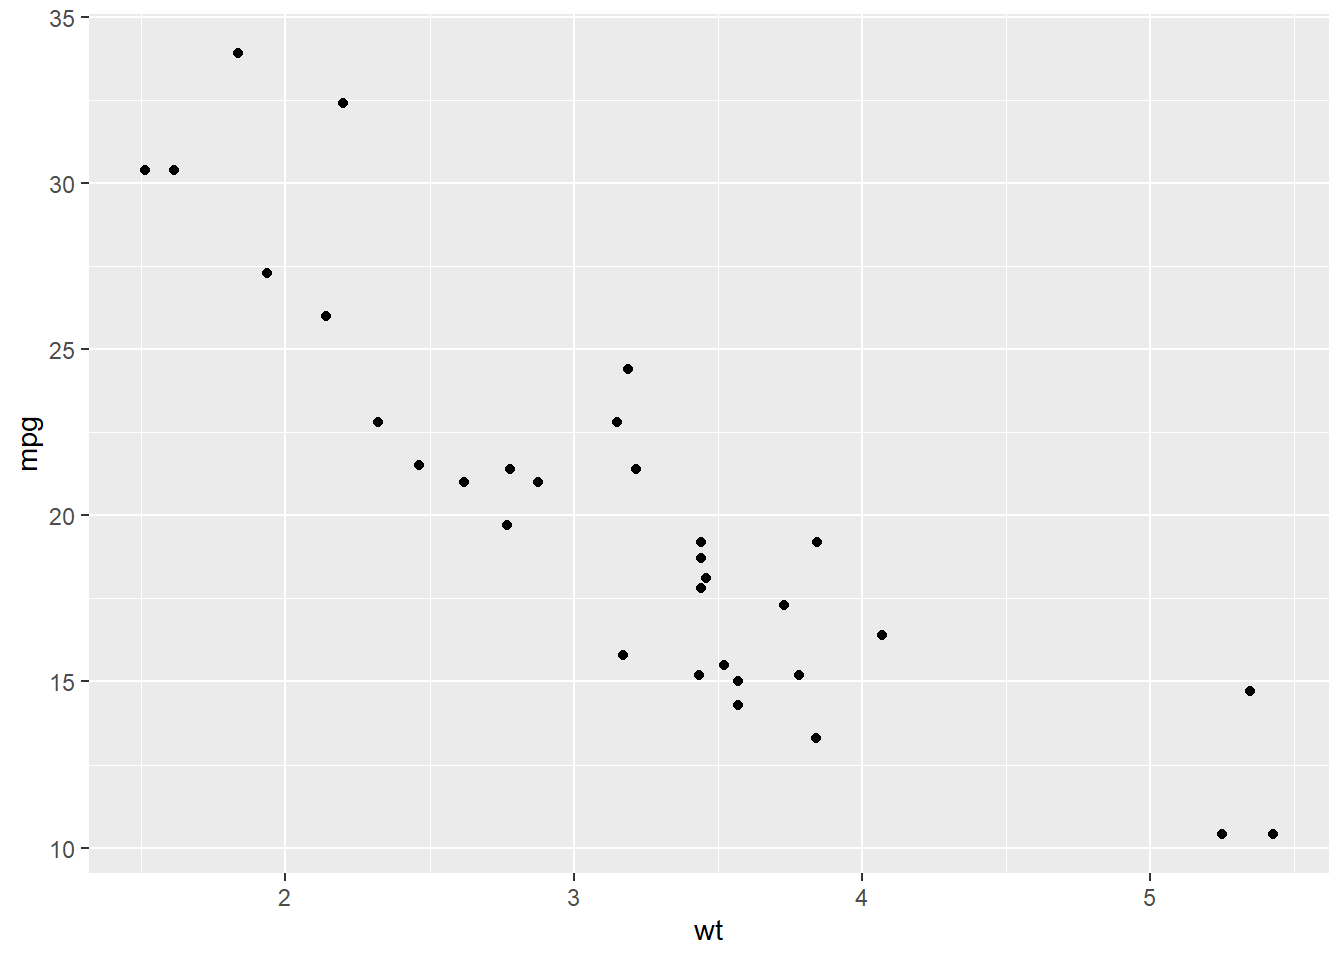
\includegraphics{RMarkDownTutorialNotes_kat_files/figure-latex/Include Figure-1.pdf}
\# Notes on Section Headers

You can see how it generates when looking at the outline area to the
right. YOU MUST INCLUDE SPACES AFTER EACH THE NUMBER OF \#\#\# YOU WANT
TO GET THE HEADING TO RENDER \# First-level

\subsection{Second Level}\label{second-level}

\paragraph{subheader under the second
level}\label{subheader-under-the-second-level}

\subsubsection{Third Level}\label{third-level}

\section{Style and Emphasis}\label{style-and-emphasis}

use the tilde key for the ``\,`'' backquote symbol. (is symbol below
tilde) to show if something is code specifically (like a function)

\texttt{ggplot()}

\emph{italic} can be used for scientific names. Use single *before and
after what you want italicized

\emph{Myadestes palmeri}

\textbf{bold} uses ** on either end of what you want bolded
\textbf{HELLO}

You can also insert blockquotes (for example a quopte that is clearly
displayed in the final document, like at the beginning of a book
chapter) Blockquotes are written after ``\textgreater{}'' example:

\begin{quote}
``I thoroughly disapprove of duels. If a man should challenge me,\\
I would take him kindly and forgivingly by the hand and lead him\\
to a quiet place and kill him.''

--- Mark Twain
\end{quote}

Again, be super careful of actually using spaces

\section{Lists}\label{lists}

\subsection{Unordered Lists}\label{unordered-lists}

\begin{itemize}
\tightlist
\item
  one item
\item
  another item
\item
  another one

  \begin{itemize}
  \tightlist
  \item
    a sub item
  \item
    another subitem
  \item
    again
  \end{itemize}
\end{itemize}

\subsection{Ordered Lists}\label{ordered-lists}

\begin{enumerate}
\def\labelenumi{\arabic{enumi}.}
\tightlist
\item
  One
\item
  Two
\item
  Three
\end{enumerate}

\begin{itemize}
\tightlist
\item
  subitem
\end{itemize}

\section{Inserting Links and
Websites}\label{inserting-links-and-websites}

\subsubsection{Not hyperlinked}\label{not-hyperlinked}

\texttt{https://abcbirds.org/bird/puaiohi}

\subsubsection{Hyperlink}\label{hyperlink}

\url{https://abcbirds.org/bird/puaiohi/}

\subsubsection{Renamed Hyperlink}\label{renamed-hyperlink}

\href{https://abcbirds.org/bird/puaiohi/}{Puaiohi (American Bird
Conservancy)}

\section{Inserting Images!}\label{inserting-images}

\#If you forgot the exclamation mark (!), it will become just a link
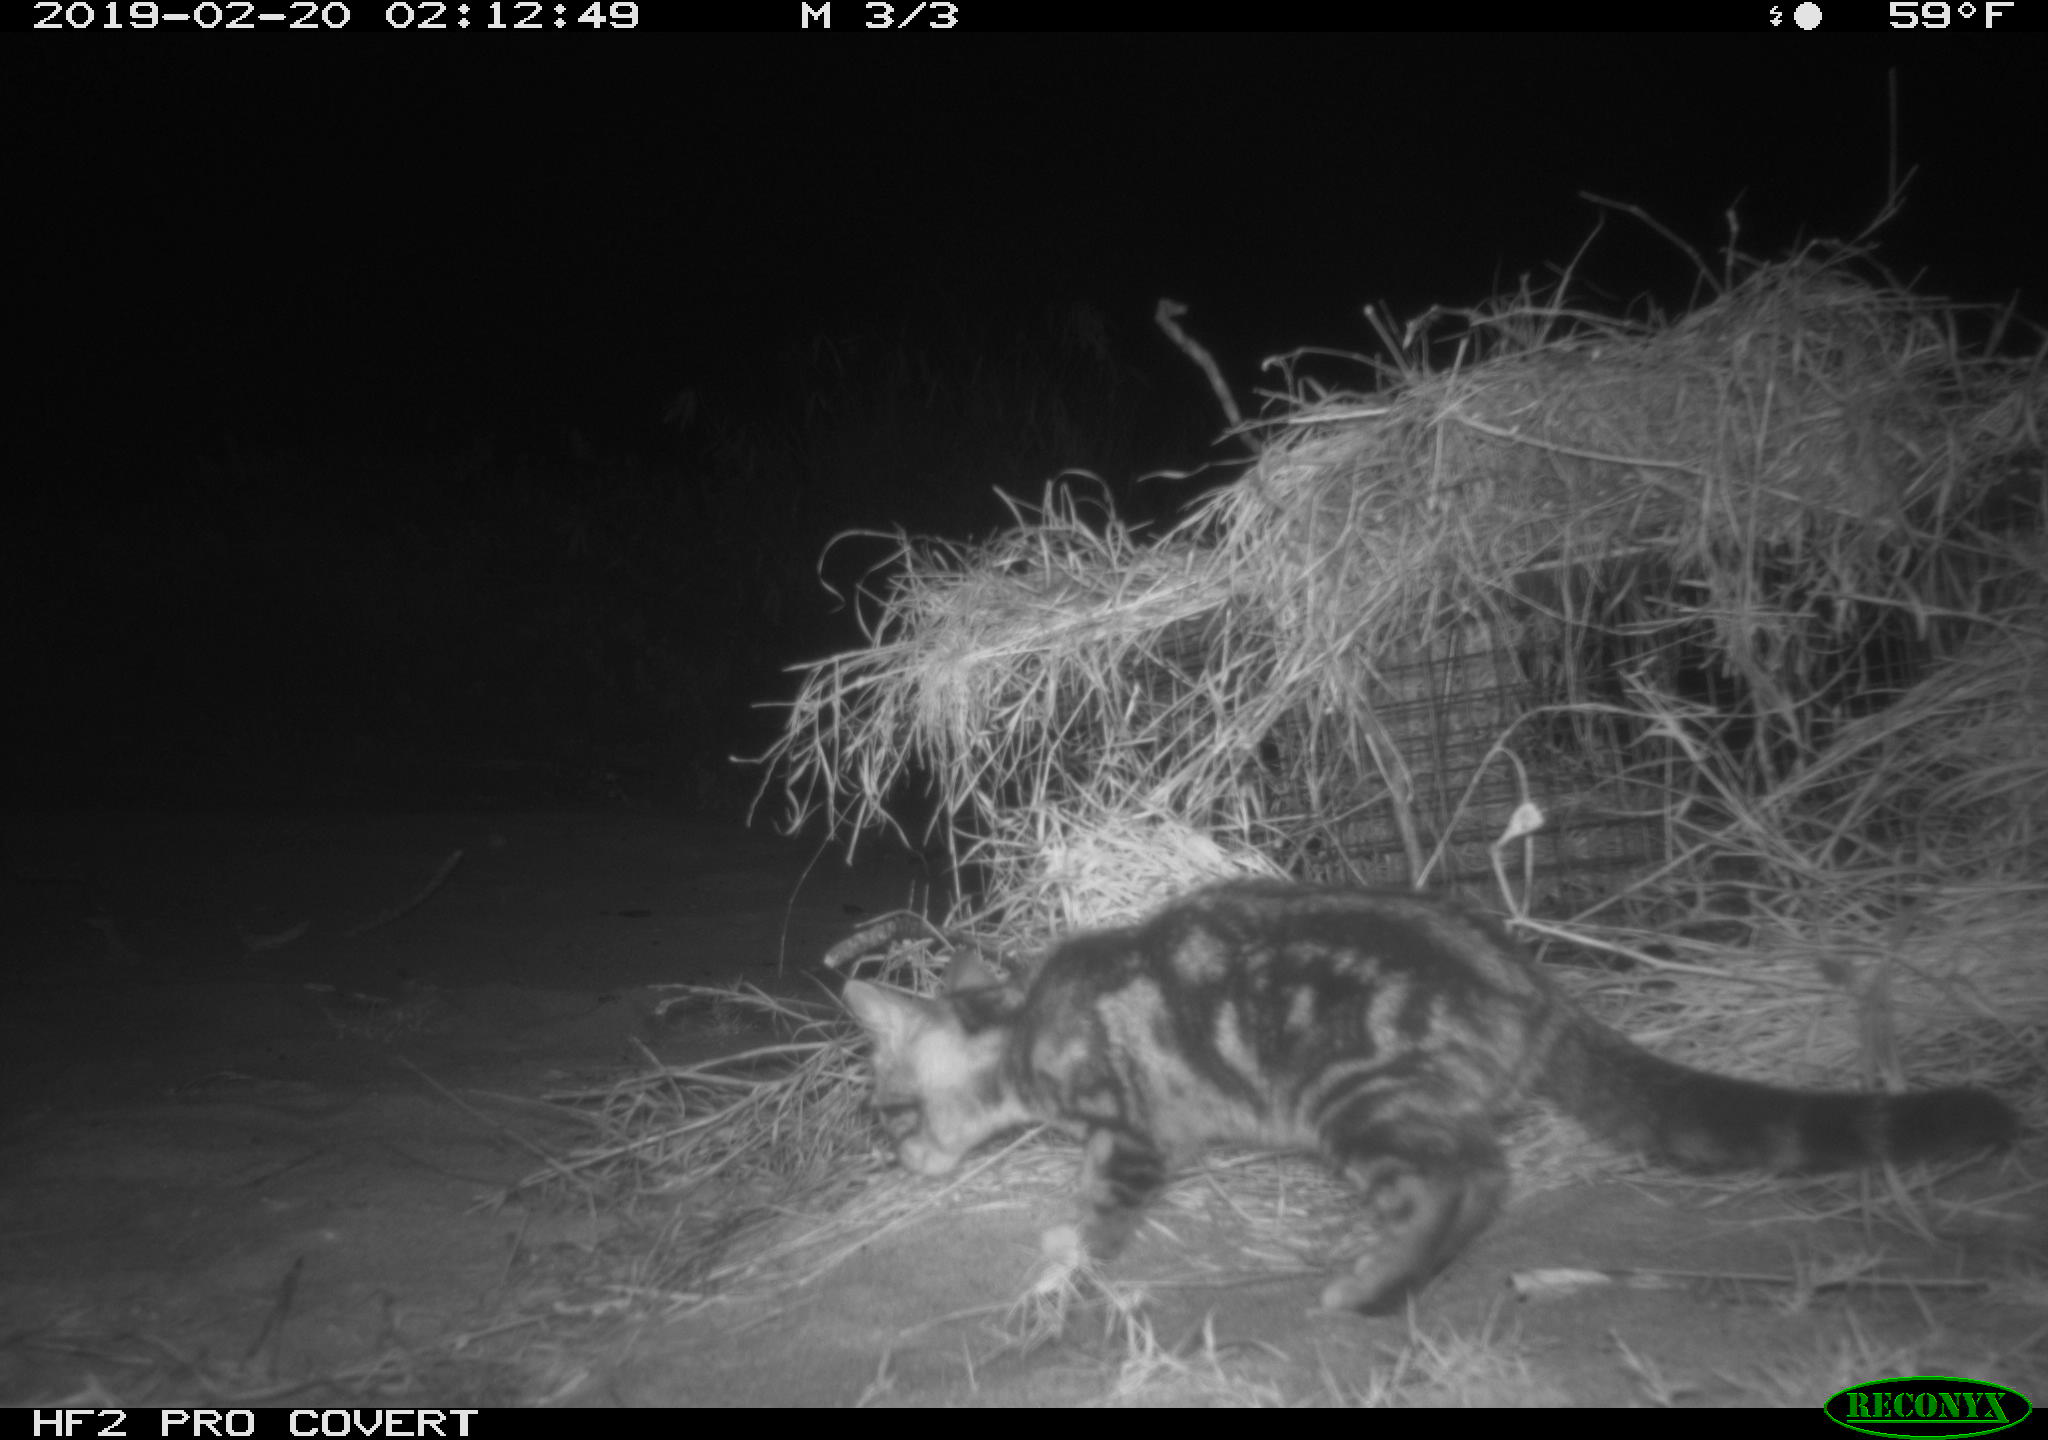
\includegraphics{RCNX0624.JPG}

\section{Creating and Formatting Tables in
Markdown}\label{creating-and-formatting-tables-in-markdown}

\begin{longtable}[]{@{}ll@{}}
\toprule\noalign{}
First Header & Second Header \\
\midrule\noalign{}
\endhead
\bottomrule\noalign{}
\endlastfoot
content cell & content cell \\
content cell & content cell \\
\end{longtable}

\subsubsection{Simpler Process Using kable
package}\label{simpler-process-using-kable-package}

\begin{Shaded}
\begin{Highlighting}[]
\FunctionTok{library}\NormalTok{(kableExtra)}
\FunctionTok{kable}\NormalTok{(}\FunctionTok{head}\NormalTok{(mtcars, }\AttributeTok{n =} \DecValTok{5}\NormalTok{), }\AttributeTok{digits =} \DecValTok{3}\NormalTok{, }\AttributeTok{format =} \StringTok{"markdown"}\NormalTok{)}\CommentTok{\#Generates table from data like the spreadsheet}
\end{Highlighting}
\end{Shaded}

\begin{longtable}[]{@{}
  >{\raggedright\arraybackslash}p{(\columnwidth - 22\tabcolsep) * \real{0.2609}}
  >{\raggedleft\arraybackslash}p{(\columnwidth - 22\tabcolsep) * \real{0.0725}}
  >{\raggedleft\arraybackslash}p{(\columnwidth - 22\tabcolsep) * \real{0.0580}}
  >{\raggedleft\arraybackslash}p{(\columnwidth - 22\tabcolsep) * \real{0.0725}}
  >{\raggedleft\arraybackslash}p{(\columnwidth - 22\tabcolsep) * \real{0.0580}}
  >{\raggedleft\arraybackslash}p{(\columnwidth - 22\tabcolsep) * \real{0.0725}}
  >{\raggedleft\arraybackslash}p{(\columnwidth - 22\tabcolsep) * \real{0.0870}}
  >{\raggedleft\arraybackslash}p{(\columnwidth - 22\tabcolsep) * \real{0.0870}}
  >{\raggedleft\arraybackslash}p{(\columnwidth - 22\tabcolsep) * \real{0.0435}}
  >{\raggedleft\arraybackslash}p{(\columnwidth - 22\tabcolsep) * \real{0.0435}}
  >{\raggedleft\arraybackslash}p{(\columnwidth - 22\tabcolsep) * \real{0.0725}}
  >{\raggedleft\arraybackslash}p{(\columnwidth - 22\tabcolsep) * \real{0.0725}}@{}}
\toprule\noalign{}
\begin{minipage}[b]{\linewidth}\raggedright
\end{minipage} & \begin{minipage}[b]{\linewidth}\raggedleft
mpg
\end{minipage} & \begin{minipage}[b]{\linewidth}\raggedleft
cyl
\end{minipage} & \begin{minipage}[b]{\linewidth}\raggedleft
disp
\end{minipage} & \begin{minipage}[b]{\linewidth}\raggedleft
hp
\end{minipage} & \begin{minipage}[b]{\linewidth}\raggedleft
drat
\end{minipage} & \begin{minipage}[b]{\linewidth}\raggedleft
wt
\end{minipage} & \begin{minipage}[b]{\linewidth}\raggedleft
qsec
\end{minipage} & \begin{minipage}[b]{\linewidth}\raggedleft
vs
\end{minipage} & \begin{minipage}[b]{\linewidth}\raggedleft
am
\end{minipage} & \begin{minipage}[b]{\linewidth}\raggedleft
gear
\end{minipage} & \begin{minipage}[b]{\linewidth}\raggedleft
carb
\end{minipage} \\
\midrule\noalign{}
\endhead
\bottomrule\noalign{}
\endlastfoot
Mazda RX4 & 21.0 & 6 & 160 & 110 & 3.90 & 2.620 & 16.46 & 0 & 1 & 4 &
4 \\
Mazda RX4 Wag & 21.0 & 6 & 160 & 110 & 3.90 & 2.875 & 17.02 & 0 & 1 & 4
& 4 \\
Datsun 710 & 22.8 & 4 & 108 & 93 & 3.85 & 2.320 & 18.61 & 1 & 1 & 4 &
1 \\
Hornet 4 Drive & 21.4 & 6 & 258 & 110 & 3.08 & 3.215 & 19.44 & 1 & 0 & 3
& 1 \\
Hornet Sportabout & 18.7 & 8 & 360 & 175 & 3.15 & 3.440 & 17.02 & 0 & 0
& 3 & 2 \\
\end{longtable}

\section{File Trees}\label{file-trees}

Need

\begin{Shaded}
\begin{Highlighting}[]
\FunctionTok{library}\NormalTok{(fs)}
\NormalTok{fs}\SpecialCharTok{::}\FunctionTok{dir\_tree}\NormalTok{ () }\CommentTok{\#generates a straight up file tree }
\end{Highlighting}
\end{Shaded}

\begin{verbatim}
## .
## +-- figure-gfm
## |   +-- Include Figure-1.png
## |   \-- pressure-1.png
## +-- figure-html
## |   \-- Include Figure-1.png
## +-- RMarkDownTutorialNotes_kat.docx
## +-- RMarkDownTutorialNotes_kat.html
## +-- RMarkDownTutorialNotes_kat.log
## +-- RMarkDownTutorialNotes_kat.md
## +-- RMarkDownTutorialNotes_kat.Rmd
## +-- RMarkDownTutorialNotes_kat.tex
## \-- RMarkDownTutorialNotes_kat_files
##     \-- figure-latex
##         \-- Include Figure-1.pdf
\end{verbatim}

\end{document}
